% Boilerplate from: https://github.com/jdavis/latex-homework-template/blob/master/homework.tex
\documentclass[table]{article}
\usepackage[table]{xcolor}
\usepackage{amssymb}
\usepackage{fancyhdr}
\usepackage{extramarks}
\usepackage{amsmath}
\usepackage{amsthm}
\usepackage{amsfonts}
\usepackage{tikz}
\usepackage{graphicx}
\usepackage{enumitem}
\usepackage{multicol}

\topmargin=-0.45in
\evensidemargin=0in
\oddsidemargin=0in
\textwidth=6.5in
\textheight=9.0in
\headsep=0.25in

\linespread{1.1}
\pagestyle{fancy}
\lhead{\hmwkAuthorName}
\chead{\hmwkTitle}
\rhead{\firstxmark}
\lfoot{\lastxmark}
\cfoot{\thepage}

\renewcommand\headrulewidth{0.4pt}
\renewcommand\footrulewidth{0.4pt}

%\setlength\parindent{15pt}%

\newcommand{\enterProblemHeader}[1]{
    \nobreak\extramarks{}{Problem \arabic{#1} continued on next page\ldots}\nobreak{}
    \nobreak\extramarks{Problem \arabic{#1} (continued)}{Problem \arabic{#1} continued on next page\ldots}\nobreak{}
}

\newcommand{\exitProblemHeader}[1]{
    \nobreak\extramarks{Problem \arabic{#1} (continued)}{Problem \arabic{#1} continued on next page\ldots}\nobreak{}
    \stepcounter{#1}
    \nobreak\extramarks{Problem \arabic{#1}}{}\nobreak{}
}

\setcounter{secnumdepth}{0}
\newcounter{partCounter}
\newcounter{homeworkProblemCounter}
\setcounter{homeworkProblemCounter}{1}
\nobreak\extramarks{Problem \arabic{homeworkProblemCounter}}{}\nobreak{}

\newenvironment{homeworkProblem}[1][-1]{
    \ifnum#1>0
        \setcounter{homeworkProblemCounter}{#1}
    \fi
    \section{Problem \arabic{homeworkProblemCounter}}
    \setcounter{partCounter}{1}
    \enterProblemHeader{homeworkProblemCounter}
}{
    \exitProblemHeader{homeworkProblemCounter}
}

\newcommand{\hmwkTitle}{Homework\ \#1}
\newcommand{\hmwkDueDate}{22 June 2020}
\newcommand{\hmwkClass}{Discrete Structures}
\newcommand{\hmwkClassTime}{Section 201}
\newcommand{\hmwkClassInstructor}{Professor Jensen}
\newcommand{\hmwkAuthorName}{\textbf{Brian Ton}}

\title{
    \vspace{2in}
    \textmd{\textbf{Discrete Structures: 1.4-1.7 Small Review}}\\
    \vspace{3in}
}

\author{\hmwkAuthorName}
\date{}

\newcommand{\solution}{\textbf{\large Solution}}

\newcolumntype{g}{>{\columncolor{yellow!20}}c}

\begin{document}
\maketitle

\pagebreak

\section{Section 1.4 Quick Review}
In the statement ``$x$ is greater than $3$,'' $x$ is called a subject and ``greater than $3$'' is called the predicate.\\
$\forall x$ means ``for all $x$.''\\
$\exists x$ means ``there exists an $x$.''\\
$P(x)$ is a propositional function that has an input $x$. Given this input, it will have a value based on if $x$ satisfies the given predicate.
\section{Example Problems for Section 1.4}
\begin{homeworkProblem}
Let $P(x)$ denote the statement ``$x \leq 4$.'' What are these truth values?
\begin{enumerate}[nosep, label=\textbf{\alph*})]
\item $P(0)$
\item $P(4)$
\item $P(6)$
\end{enumerate}
\subsection{Solution}
\begin{enumerate}[nosep, label=\textbf{\alph*})]
\item \textbf{T}\\
In this case, $x$ would be 0, which is less than or equal to 4.\\
Therefore, the answer to this would be \textbf{T}.
\item \textbf{T}
\item \textbf{F}
\end{enumerate}
\end{homeworkProblem}
\begin{homeworkProblem}
Suppose that the domain of the propositional function $P(x)$ consists of the integers $-2$, $-1$, $0$, $1$, and $2$.
Write out the proposition using disjunctions, conjunctions, and negations.\\
$\exists x \neg P(x)$
\subsection{Solution}
\textbf{\(\neg P(-2) \lor \neg P(-1) \lor \neg P(0) \lor \neg P(1) \lor \neg P(2)\)}\\
Here, $\exists x \neg P(x)$ means that ``there exists an $x$ such that $\neg P(x)$ is true.'' Therefore, it follows that at least one element in the domain satisfies $\neg P(x)$, which leads to the solution (where we use the ``or'' operator because we are looking for existence, which is true if one of the terms in the statement is true).
\end{homeworkProblem}
\begin{homeworkProblem}
Translate the statement into logical expressions using predicates, quantifiers, and logical connectives.\\
One of your tools is not in the correct place, but it is in excellent condition.
\subsection{Solution}
$\exists x(\neg P(x) \land C(x))$ where $x$ is a tool in the toolbox, $P(x)$ means that tool $x$ is in the correct position, and $C(x)$ means that the tool is in excellent condition.\\
The key to this problem is utilizing the existential operator, as the problem is stating that ``One of your tools'' satisfies the conditions, implying the use of the existential operator. The rest then is similar to Section 1.1 where we translated propositional logic.
\end{homeworkProblem}
\begin{homeworkProblem}
Express the statement using quantifiers. Then form the negation of the statement. Next, express the negation in simple English.\\

There is someone in this class who does not have a good attitude.
\subsection{Solution}
\textbf{Given statement:}\\
\(
\exists x(\neg A(x))
\)
where $A(x)$ means that $x$ has a good attitude.\\
\textbf{Negation:}\\
\(
\neg \exists x(\neg A(x)) \equiv \forall x(A(x))
\)\\
(Note the use of De Morgan's Law for Quantifiers that flips the ``there exists'' into a ``for all'' and negates the inside)\\
\textbf{In simple English:}\\
Everyone in the class has a good attitude.
\end{homeworkProblem}
\setcounter{homeworkProblemCounter}{1}

\section{Section 1.5 Quick Review}
Pretty much the same as 1.4 except with multiple quantifiers.
Examples:
\(\forall x \forall y\) means ``for all x and y.''\\
\(\forall x \exists y\) means ``for all $x$ there exists $y$.''\\
\(\exists x \forall y\) means ``there exists an $x$ such that for all $y$.''
\begin{homeworkProblem}
Translate the statement into English, where the domain for each variable consists of all real numbers.
$\forall x \forall y(((x \geq 0) \land (y \geq 0)) \rightarrow (xy \geq 0))$
\subsection{Solution}
For all real numbers x and y, if x is greater than equal to 0 and y is greater than equal to 0, then x times y is greater than or equal to 0.
\end{homeworkProblem}
\begin{homeworkProblem}
Let $I(x)$ be the statement ``x has an internet connection.'' Write the below statement using quantifiers.
Everyone except one student in your class has an internet connection.
\subsection{Solution}
\(
\exists x(\neg I(x) \land \forall y (x \neq y \rightarrow I(y))
\)\\
This can be thought of as ``there exists a student x such that x does not have an internet connection and every other student except them has one.''
\end{homeworkProblem}
\begin{homeworkProblem}
Rewrite the statement.\\
$\neg \exists y(\exists xR(x,y) \lor \forall xS(x,y)$\\
\subsection{Solution}
\begin{align*}
\neg \exists y(\exists xR(x,y) \lor \forall xS(x,y))
&{\equiv} \forall y \neg(\exists xR(x,y) \lor \forall xS(x,y) && \text{(De Morgan's Law of Quantifiers)}\\
&{\equiv} \forall y (\neg \exists xR(x,y) \land \neg \forall xS(x,y) && \text{(De Morgan's Law)}\\
&{\equiv} \forall y (\forall x \neg R(x,y) \land \exists x \neg S(x,y)) && \text{(De Morgan's Law of Quantifiers)}
\end{align*}
\end{homeworkProblem}
\setcounter{homeworkProblemCounter}{1}
\section{Section 1.6 Quick Review}
Nothing much here, you just need to know the rules of inference from pages 76, 80.\\
Also, there are a couple of fallacies you must know, especially \textbf{inverse} and \textbf{converse} error.\\
An example of each is given below.\\
Converse Error:\\
\(
p \rightarrow q\\
q\\
\therefore p
\)\\~\\
Inverse Error:\\
\(
p \rightarrow q\\
\neg p\\
\therefore \neg q
\)
\begin{homeworkProblem}
Use the rules of inference to show that if $\forall x (P(x) \rightarrow (Q(x) \land S(x))$ and $\forall x(P(x) \land R(x))$ are true, then $\forall x(R(x) \land S(x))$ is true.
\subsection{Solution}
(I couldn't find a way to type this up, so I scanned my writing)
\begin{figure}[h!]
	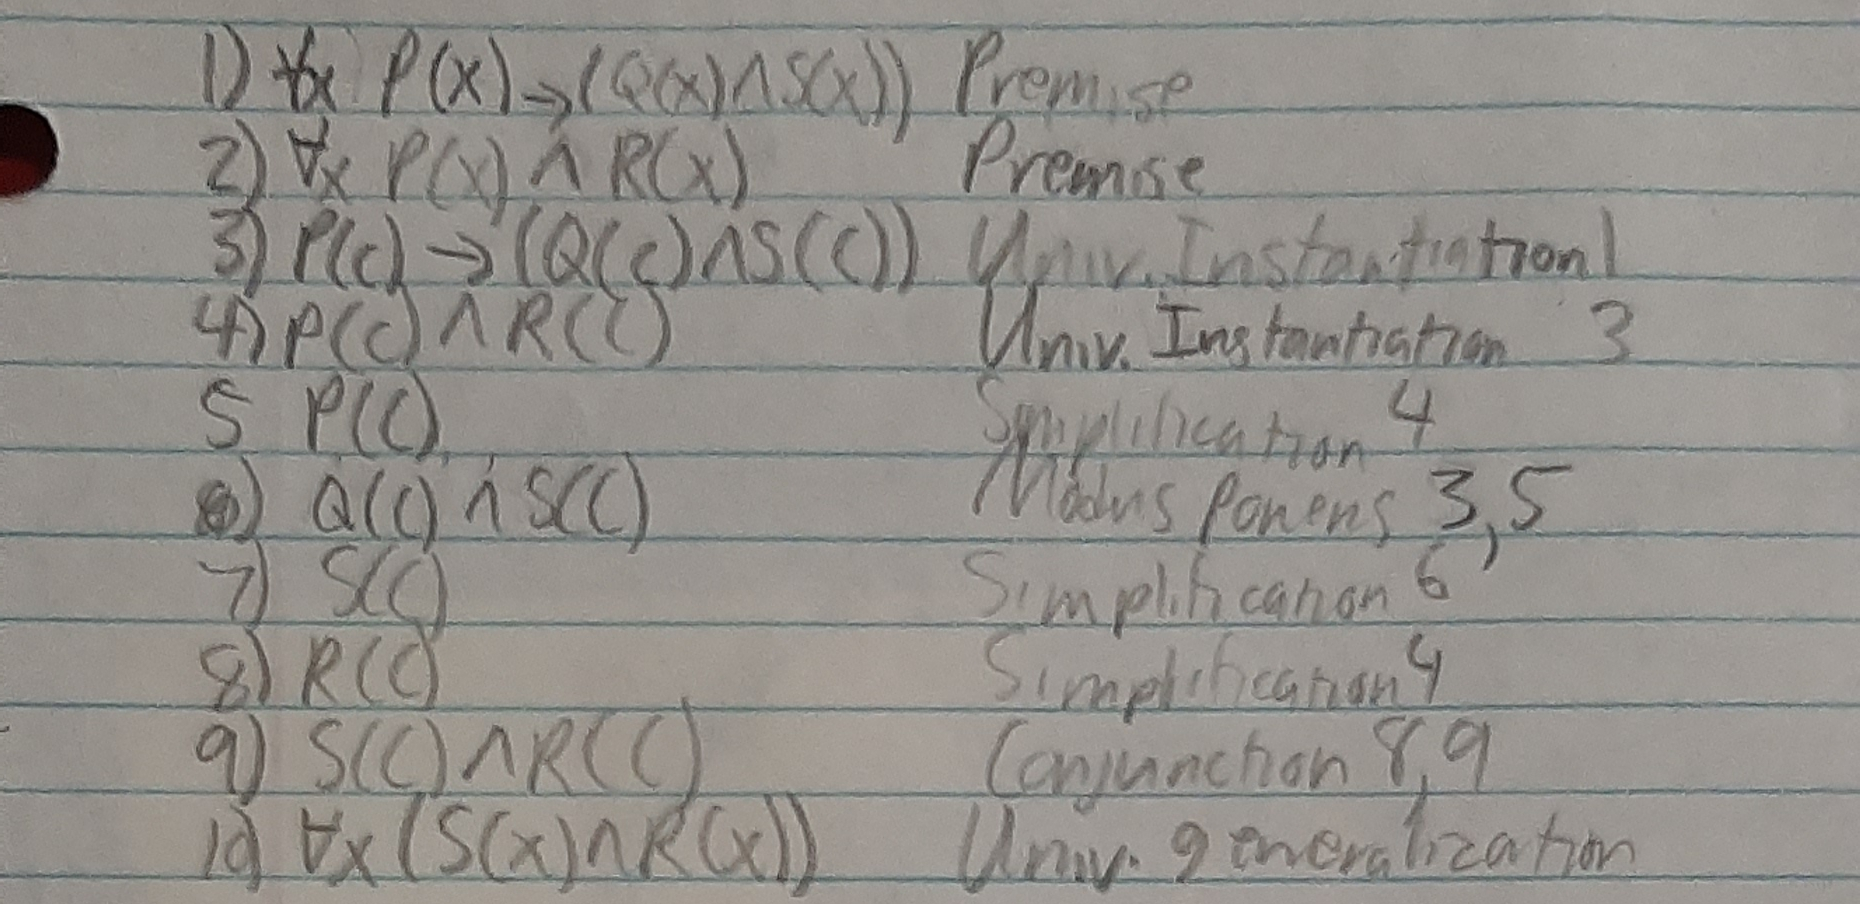
\includegraphics[scale=.15]{images/Prob1-6_1.jpg}
\end{figure}
\end{homeworkProblem}
\end{document}